%!TEX root = ../zeeman.tex
В 1896 г. Зееман обнаружил, что спектральные линии определенным образом расщепляются, если источник света поместить в магнитное поле. При наблюдении поперек поля спектральная линия расщепляется на три линейно поляризованные компоненты. Средняя компонента не смещена, крайние смещены в противоположные стороны на одинаковые расстояния (в шкале частот). Смещение пропорционально напряженности внешнего магнитного поля \textbf{B}. В средней компоненте электрический вектор направлен параллельно магнитному полю (такие компоненты называются $\pi-$компонентами), в крайних - перпендикулярно к нему(такие компоненты называются $\sigma-$компонентами). Интенсивность $\pi-$компоненты вдвое, а каждой из $\sigma-$компонент в четыре раза меньше интенсивности исходной линии. 

При наблюдении вдоль магнитного поля получается такое же смещение (при одинаковой напряженности магнитного поля), что и в предыдущем случае, но несмещенная компонента отсутствует. Интенсивность каждой компоненты вдвое меньше интенсивности исходной спектральной линии. Обе компоненты поляризованы по кругу в противоположных направлениях (их принято называть также $\sigma-$компонентами). Если свет распространяется в направлении магнитного поля, то $\sigma-$компонента с меньшей частотой поляризована по правому, с большей - по левому кругу. При изменении направления магнитного поля на противоположное меняется на противоположную и круговая поляризация обеих компонент.
 
 Описанная картина расщепления спектральных линий объясняется классической теорией Лорентца. Как и классическая теория дисперсии, это есть модельная теория, в простейшей форме которой излучающими центрами являются гармонические осцилляторы в виде квазиупругосвязанных электронов. В отсутствие внешнего магнитного поля уравнение движения таокгор электрона имеет вид $\ddot{\vec{r}}-\omega_0^2 \vec{r}=0$, где $\omega_0$ - собственная частота электрона. При наличии постоянного магнитного поля на электрон действует еще сила Лорентца $\vec{F_l}=-\frac ec[\dot{\vec{r}}, \vec{B}]$. Уравнение движения электрона принимает вид: $$\ddot{\vec{r}}-\omega_0^2 \vec{r}=-\frac{e}{mc}[\dot{\vec{r}}, \vec{B}],$$ где m - масса электрона. Введя ларморовскую частоту $$\Omega=\frac{e}{2mc}\vec{B},$$ приведем его к виду $$\ddot{\vec{r}}+2[\dot{\vec{r}},\vec{\Omega}]+\omega_0^2\vec{r}=0.$$
 Классическая теория сводится к решению этого уравнения. Перейдем к системе трех скалярных уравнений $$\ddot{x}+2\Omega \dot{x}+\omega_0^2x=0,$$ $$\ddot{y}+2\Omega \dot{y}+\omega_0^2y=0,$$ $$\ddot{z}+\omega_0^2z=0.$$
Из последнего уравнения видно, что магнитное поле не влияет на движение электрона вдоль магнитного поля. Это и понятно, так как при таком движении не возникает силы, действующей со стороны магнитного поля. Интегрирование двух первых уравнений удобно провести в комплексной форме. Объединим: $\zeta=x+iy$, $-i\dot{\zeta}=\dot{y}-i\dot{x}$, умножим второе уравнение на i и сложим с первым. Тогда $$\ddot{\zeta}-i2\Omega\dot{\zeta}+\omega_0^2\zeta=0.$$Ищем решение уравнения  в виде $\zeta=e^{i\omega t}$. Постоянная $\omega$ найдется из квадратного уравнения $\omega^2+2\Omega \omega+\omega_0^2=0,$ которое дает $$\omega=\Omega \pm \sqrt{\omega_0^2+\Omega^2}.$$ Даже в очень сильных магнитных полях квадратом ларморовской частоты можно пренебречь по сравнению с $\omega_o^2$. С большой точностью $\omega=\pm \omega_0+\Omega$. Переобозначим: $\omega_1=\omega_0+\Omega$, $\omega_2=\omega_0-\Omega$. Тогда $$\zeta_1=e^{i\omega_1 t}, \zeta_2=e^{i\omega_2 t}.$$

\begin{figure}[h]
	\centering
	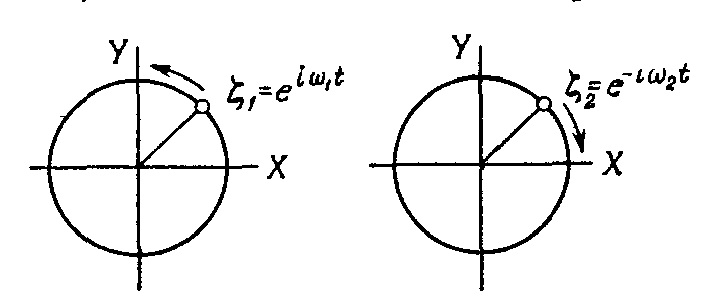
\includegraphics[width=0.4\linewidth]{fig/fig11}
\end{figure}

Первое решение представляет круговое движение, в котором электрон вращается против часовой стрелки с угловой частотой $\omega_1$, второе - также круговое движение, но по часовой стрелке и с частотой $\omega_2$. Общее решение соответствует наложению таких двух вращений и представляется в виде $\zeta=C_1\zeta_1+C_2\zeta_2$, где $C_1$ и $C_2$ - произвольные постоянные.

Согласно квантовой теории излучения энергия атома $E$ может принимать лишь дискретные строго определенные значения. Совокупность таких разрешенных значений (уровней энергии) называют \textbf{энергетическим спектром атома}. Энергетический спектр атома может быть задан с помощью вполне определенного набора внутренних характеристик атома - его \textbf{квантовых чисел}. Наиболее точный смысл каждого квантового числа выясняется при решении \textbf{уравнения Шредингера}, в котором квантовые числа определяют \textbf{спектр собственных значений}. Мы же введем лишь названия и обозначения, а там, где это возможно, дадим краткую, более или менее наглядную и нс слишком строгую, характеристику квантовых чисел атома:

$n$ -- \textbf{главное квантовое число}, определяющее среднее расстояние электронного облака от ядра;

$L$ -- \textbf{орбитальное квантовое число}, характеризующее сумму моментов импульса электронов $\vec{P_L}$, связанных с их вращением вокруг ядра;

$S$ -- \textbf{спиновое квантовое число}, описывающее сумму собственных моментов импульса электронов $\vec{P_S}$, не связанных с их вращением вокруг ядра\footnote{Наличие собственною механического момента (спина) и магнитного момента у покоящегося электрона не имеет удовлетворительного наглядного толкования и должно восприниматься как факт, однозначно следующий из результатов многочисленных экспериментов.};

$J$ -- \textbf{азимутальное квантовое число}, которому ставится в соответствие полный механический момент электронов в атоме:

\begin{equation}
	\vec{P_J}=\vec{P_L}+\vec{P_S}
	\label{eq:1}
\end{equation}

$M_J$ -- \textbf{магнитное квантовое число}, название которого связано с тем, что энергия атома зависит от $M_J$ лишь при наличии внешнего магнитного поля: $E(n,J,L,S,M_J)$. В отсутствии магнитного поля для всех допустимых значений $M_J$ энергия атома имеет одно и то же значение $E(n,J,L,S,M_J)$ -- в этом случае говорят, что имеет место \textbf{вырождение} (неоднозначность) состояния атома по квантовому числу $M_J$. Из элементарной физики известно, что в магнитном поле могут изменить свою энергию лишь системы, имеющие (или приобретающие) \textbf{магнитный момент} $\vec{\mu}$, причем изменение энергии равно:

\begin{equation}
	\delta E=-(\vec{\mu}\vec{H})=-\mu_HH.
	\label{eq:2}
\end{equation}

Из сказанного ясно, что квантовое число $M_J$ характеризует проекцию магнитного момента атома $\vec{\mu}$ на направление внешнего магнитного поля $\vec{H}$.

\begin{figure}[tb]
	\centering
	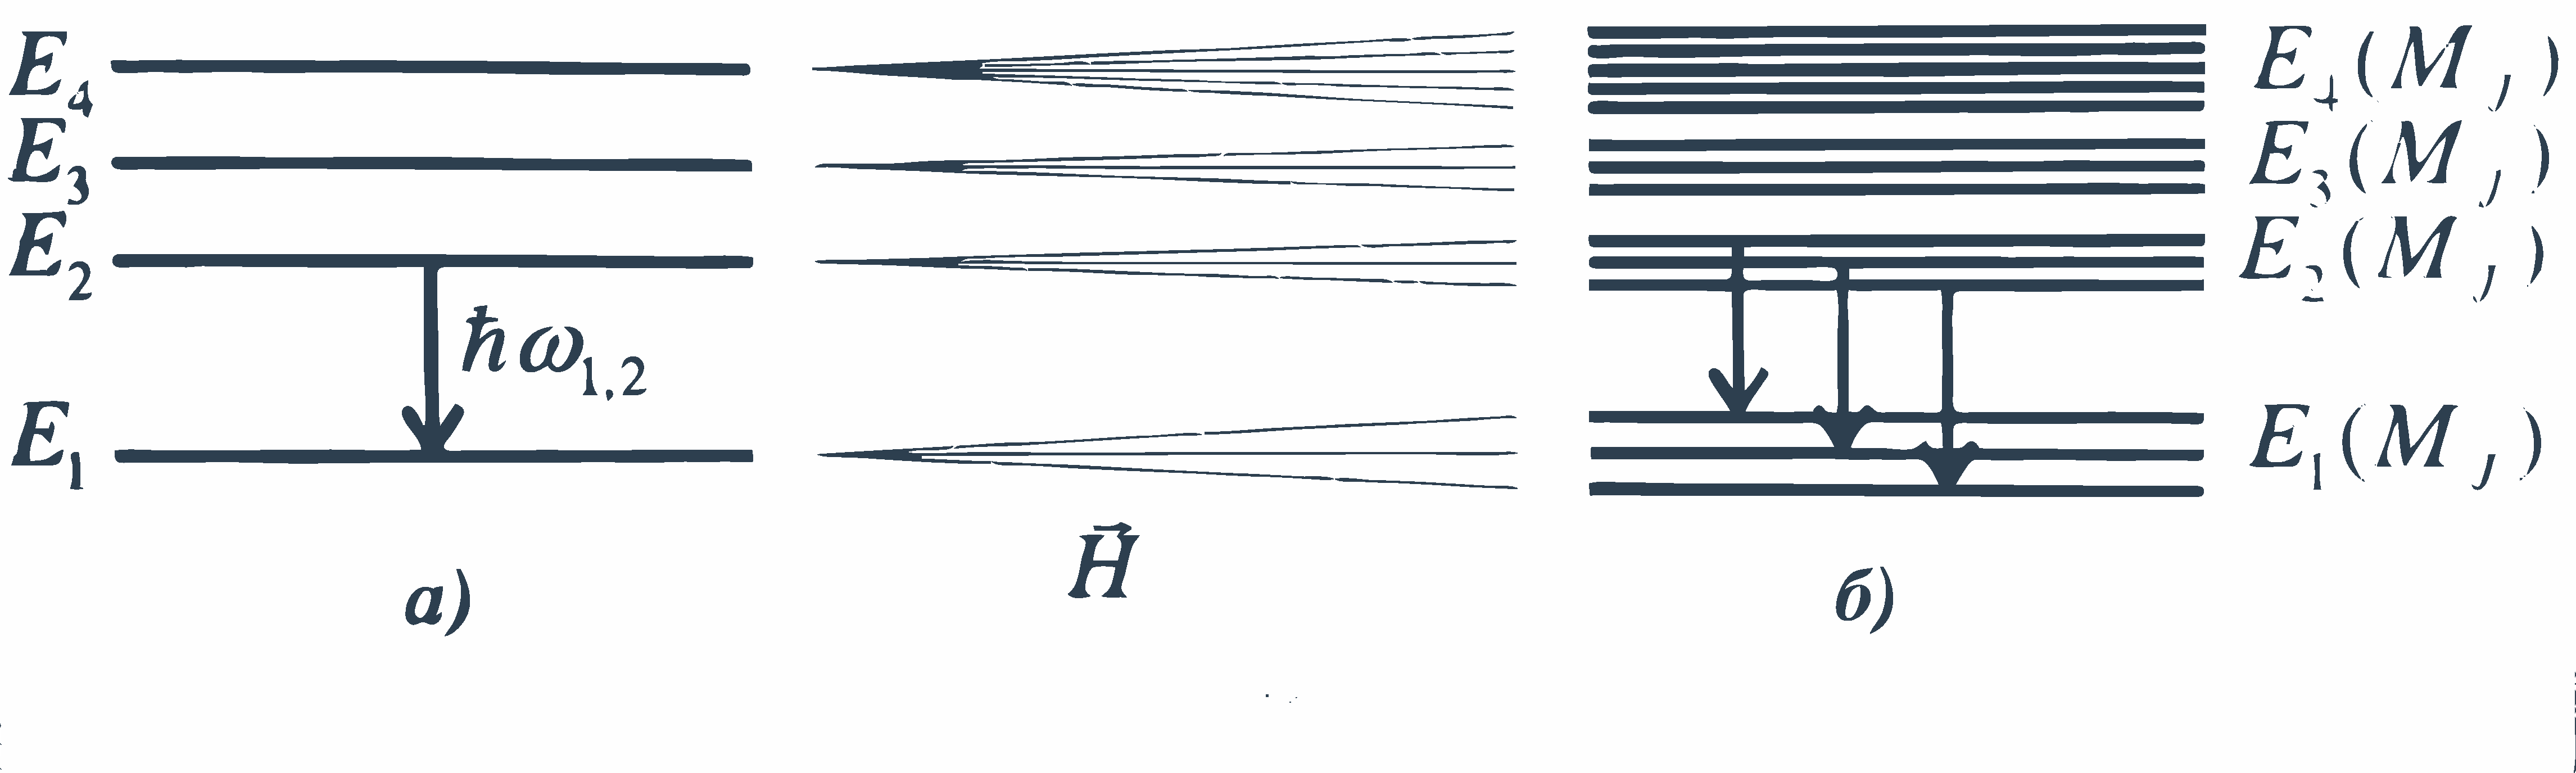
\includegraphics[width=\linewidth]{fig/fig1}
	\caption{Энергетическая структура атома и некоторые из возможных излучательных переходов
	а) в невозмущенном состоянии, б) при наложении внешнего магнитного поля}
	\label{fig:1}
\end{figure}

При переходе атома с более высокого энергетического уровня $E_2$ на более низкий $E_1$, излучается квант электромагнитной энергии (\ref{fig:1}) с частотой

\begin{equation}
\omega_{1,2}=\frac{E_2-E_1}{\hbar}
\label{eq:3}
\end{equation}
где $\hbar = 1.054\cdot10^{-27}$ эрг$\cdot$с -- постоянная Планка. Поскольку при наложении внешнего магнитного поля вырождение энергетических состояний $E_2$ и $E_1$ по квантовому числу $M_J$ снимается (т.е. происходит расщепление каждого энергетического уровня на несколько подуровней), в спектре излучения мы вместо одной наблюдаем несколько частот (линий) излучения (\ref{fig:1}). Этот эффект расщепления спектральных линий атомов в магнитном поле и называется \textbf{эффектом Зеемана}.

Точное решение уравнение Шредингера может быть найдено лишь в небольшом числе простейших случаев. Предположим, что гамильтониан данной физической системы имеет вид:
$$\widehat{H}=\widehat{H_0}+\widehat{V},$$
где $\widehat{V}$ представляет собой малую поправку к "невозмущенному" оператору $\widehat{H_0}$. Рассматриваются возмущения, не зависящие явно от времени.

Задача теории возмущений для дискретного спектра может быть сформулирована следующим образом. Предполагается, что собственные функции $\psi_n^{(0)}$ и собственные значения оператора $\widehat{H_0}$ известны, т.е известны точные решения уравнения

$$\widehat{H_0}\psi^{(0)}=E^{(0)}\psi{(0)}.$$

Требуется найти приближенные значения уравнения

$$\widehat{H}\psi=(\widehat{H_0}+\widehat{V})\psi=E\psi,$$
т.е приближенные выражения для собственных функций $\psi_n$ и значений $E_n$ возмущенного оператора $\widehat{H}$. Все собственные значения оператора $\widehat{H_0}$ не вырождены.

Разложим искомую функцию $\psi$ по функциям $\psi^{(0)}_m$:

$$\psi=\sum_m C_m \psi^{(0)}_m.$$

$$\sum_m C_m(E_m^{(0)}+\widehat{V})\psi_m^{(0)}=\sum_m C_mE\psi_m^{(0)},$$
умножив равенство с обеих сторон на $\psi_k^{(0)*}$ и интегрируя:

$$(E-E_k^{(0)})C_k=\sum_m V_{km}C_m.$$

Здесь введена матрица $V_{km}$ оператора возмущения $\widehat{V}$, определенная с помощью невозмущенных функций $\psi_m^{(0)}$:

$$V_{km}=\int \psi_k^{(0)*} \widehat{V} \psi_m^{(0)} dq.$$
будем искать значения коэффициентов $C_m$ и энергии Е в виде рядов

$$E=E^{(0)}+E^{(1)}+E^{(2)}+..., C_m=C_m^{(0)}+C_m^{(1)}+C_m^{(2)}+...,$$
где величины $E^{(1)}, C_m^{(1)}$ - того же порядка малости, что и возмущение $\widehat{V}$, величины $E^{(2)}, C_m^{(2)}$ - второго порядка малости и т.д. 

Определим поправки к n-му собственному значению и собственной функции, соответственно чему полагаем $C_n^{(0)}=1, C_m^{(0)}=0, m\neq n$. Для отыскания первого приближения учтем, что $E=E_n^{(0)}+E_n^{(1)}, C_k=C_k^{(0)}+C_k^{(1)}$, сохранив только члены первого порядка. Уравнение с $k=n$ дает:

$$E_n^{(1)}=V_{nn}=\int \psi_k^{(0)*} \widehat{V} \psi_n^{(0)} dq.$$

Таким образом, поправка первого приближения к собственному значению $E_n^{(0)}$ равна среднему значению возмущения в состоянии $\psi_n^{(0)}$. 

При $k\neq n$: $C_k^{(1)}=\frac{V_{kn}}{E_n^{(0)}-E_k^{(0)}}$, a $C_n^{(1)}$ остается произвольным и должно быть выбрано так, чтобы функция $\psi_n=\psi_n^{(0)}+\psi_n^{(1)}$ была нормирована с точностью до членов первого порядка включительно. Для этого надо положить $C_n^{(1)}=0$. Действительно, функция
$$\psi_n^{(1)}=\sum_{m,m\neq n} \frac{V_{mn}}{E_n^{(0)}-E_m^{(0)}}\psi_m^{(0)}$$
ортогональна к $\psi_n^{(0)}$, а поэтому интеграл от $|\psi_n^{(0)}-\psi_n^{(1)}|^2$ отличается от единицы лишь на величину второго порядка малости. Так определяется поправка первого приближения к волновым функциям.

Должно иметь место  неравенство

$$|V_{mn}|\ll|E_n^{(0)}-E_m^{(0)}|,$$
т.е матричные элементы возмущения должны быть малы по сравнению с соответствующими разностями невозмущенных уровней энергии.

Определим еще поправку второго приближения к собственному значению $E_n^{(0)}$. Для этого полагаем $E=E_n^{(0)}+E_n^{(1)}+E_n^{(2)}, C_k=C_k^{(0)}+C_k^{(1)}+C_k^{(2)}$ и рассматриваем члены второго порядка малости. Уравнение с $k=n$ дает

$$E_n^{(2)}C_n^0=\sum_{m,m\neq n} V_{nm}C_m^{(1)},$$
откуда

$$E_n^{(2)}=\sum_{m,m\neq n} \frac{|V_{mn}|^2}{E_n^{(0)}-E_m^{(0)}}$$
(воспользовались тем, что в силу эрмитовости оператора $\widehat{V}: V_{mn}=V_{nm}^*$).

Отметим, что поправка второго приближения к энергии нормального состояния всегда отрицательна. Если $E_n^{(0)}$ соответствует наименьшему значению, то все члены в сумме отрицательны.

Дальнейшие приближения можно вычислить аналогичным образом.
